\section{Ejercicio 4}
La asortatividad/homofilia es la tendencia de un nodo, de una red, se conecte con otros 
de caracteristicas similares, esto en terminos mathematicos es evaluar la correlaci\'on
de links entre nodos del mismo tipo \citep{newman2003}. Esta propiedad tiende a ser caracteristica 
para tipos de redes distintas: En redes de amistad por ejemplo se tiende a hacer uniones entre
nodos \textit{parecidos}, mientras que en redes biologicas, los \textit{hubs} tienes a evadirse 
entre ellos y asociarse con nodos de menor grado \citep{newman,barabasi}. 

En este ejercicio se plantea evaluar la asortatividad de cuatro redes (dos sociales y dos biol\'ogicas) a trav\'es
de dos m\'etodos distintos: Mediante la estimaci\'on de la correlaci\'on de grado a partir del grado medio del
vecindario de un nodo \citep{barabasi}; y a trav\'es del Coeficiente de Correlaci\'on de Grado propuesto por Newman
\citep{newman2003,newman}.

\subsection{Consideraciones generales}
\begin{figure}[!ht]
    \centering
    \begin{subfigure}[b]{0.30\columnwidth}
        \includegraphics[width=\textwidth]{./schemes/netscience-gml.pdf}
        \caption{\label{fig4:NETSCIENCE}NETSCIENCE}
    \end{subfigure}
    \begin{subfigure}[b]{0.30\columnwidth}
        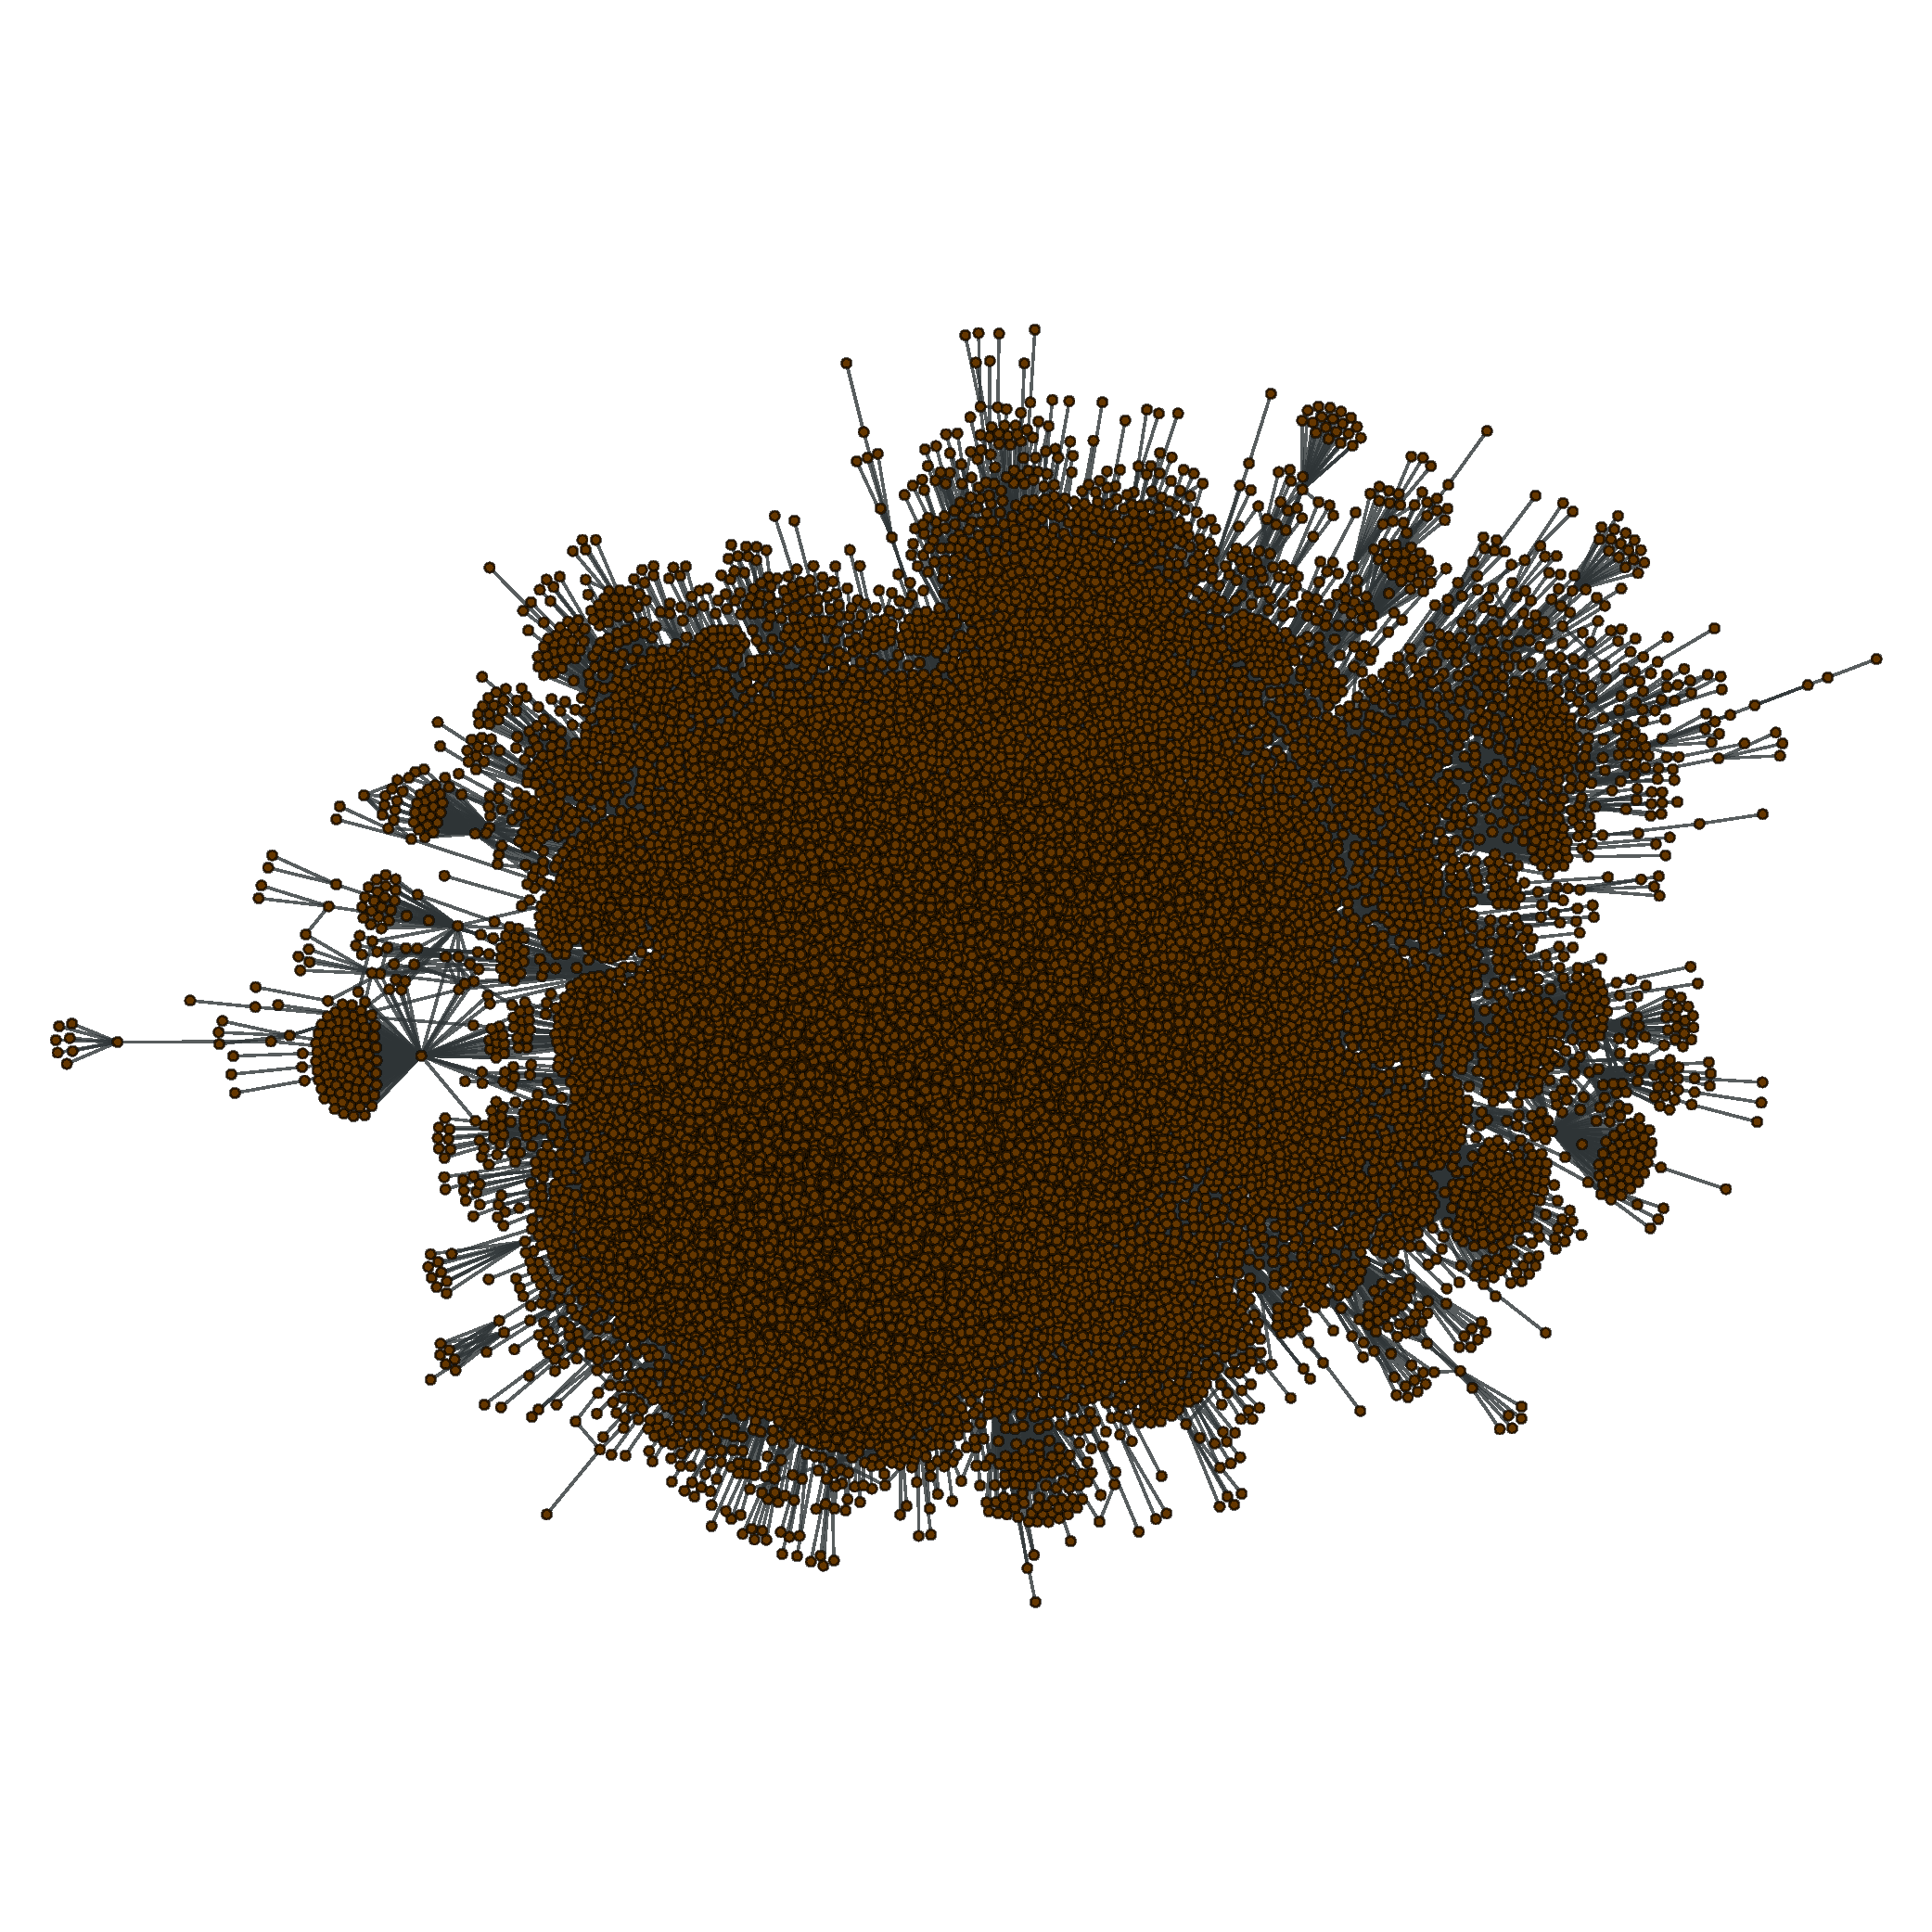
\includegraphics[width=\textwidth]{./schemes/as-22july06-gml.pdf}
        \caption{\label{fig4:WWW}WWW}
    \end{subfigure}
    \\
    \begin{subfigure}[b]{0.30\columnwidth}
        \includegraphics[width=\textwidth]{./schemes/yeast_AP-MS-txt.pdf}
        \caption{\label{fig4:ap_ms} AP-MS}
    \end{subfigure}
    \begin{subfigure}[b]{0.30\columnwidth}
        \includegraphics[width=\textwidth]{./schemes/yeast_Y2H-txt.pdf}
        \caption{\label{fig4:y2h} Y2H}
    \end{subfigure}
    \caption{\label{fig4:grafos}\textit{Layout} SFDP para cada red estudiada \\
    (script \texttt{plot.py~<archivo>\quad-f <fmt>}).}
\end{figure}
Consideremos las redes de colaboraciones cientificas (NETSCIENCE), red de internet (WWW) y dos redes de levadura analizadas 
en el ejercicio 1 (AP-MS y Y2H), las cuales son mostradas en la figura \ref{fig4:grafos}.


Un m\'etodo alternativo para 
evaluar asortividad es analizar la matriz de correlaci\'on entre grados (\textit{mixing matrix}) la cual se presenta en
la figura \ref{fig4:mix}.


\begin{figure}[!ht]
    \centering
    \begin{subfigure}[b]{0.45\columnwidth}
        \includegraphics[width=\textwidth]{./schemes/mixing_netscience-gml.pdf}
        \caption{\label{fig4:NETSCIENCE}NETSCIENCE}
    \end{subfigure}
    \begin{subfigure}[b]{0.45\columnwidth}
        \includegraphics[width=\textwidth]{./schemes/mixing_as-22july06-gml.pdf}
        \caption{\label{fig4:WWW}WWW}
    \end{subfigure}
    \\
    \begin{subfigure}[b]{0.45\columnwidth}
        \includegraphics[width=\textwidth]{./schemes/mixing_yeast_AP-MS-txt.pdf}
        \caption{\label{fig4:ap_ms} AP-MS}
    \end{subfigure}
    \begin{subfigure}[b]{0.45\columnwidth}
        \includegraphics[width=\textwidth]{./schemes/mixing_yeast_Y2H-txt.pdf}
        \caption{\label{fig4:y2h} Y2H}
    \end{subfigure}
    \caption{\label{fig4:mix} Mixing Matrix para cada caso. En la red WWW se ha ajustado los limites de gr\'afico
    de manera que sean visibles las correlaciones de bajo grado
    \\(script \texttt{degree\_mixing\_plot.py <archivo>\quad-f <fmt>})}
\end{figure}

De la figura se puede observar que, para todos los casos, la mayor densidad de correlaci\'on se puede encontrar en los 
grados peque\~nos, pero no es claro como se propaga esta correlaci\'on para grados mayores debido a que tiende rapidamente 
a cero. A\'un m\'as, no es posible hacer una comparaci\'on clara entre cada red a partir de sus respectivas matrices. Motivados por estas razones evaluamos otras m\'etodologias.

\subsection{Grado medio del vecindario $k_{nn}$ (revising \citet{barabasi})}
En esta metodolog\'ia estamos interesados en analizar el comportamiento de los vecinos de un nodo de grado $k$, para
ello consideramos el grado medio de los vecinos $k_{nn}$ de un nodo de grado $k$, esto es
\begin{align}
    k_{nn}(k) = \sum_{k'} k' P(k'|k)
\end{align}
este promedio est\'a hecho sobre la probabilidad de que: dado un nodo de grado $k$, tenga un vecino de grado $k'$.


\subsection{Coeficiente de Correlaci\'on de Grado}
